\section{Introduction}

For this thesis a Java library called \verb|gp-modifiable-ast| was implemented. 
\verb|gp| stands for general purpose, meaning that it can provide the API for different grammars, e.g. for different programming languages.

\subsection{Motivation}

The motivation for this work came from a practical problem. 
During the development of a large enterprise web application, there was a need to change the translation system.
A translation system receives a token as a string and returns a predefined translation depending on the target language.
This caused some problems because the new translation system had a different call syntax than the old one.
This refactoring required looking at external data stored in a database for each different call to the translation function.
Because of the dependency on external data, the automatic tools provided by the IDE were not sufficient to refactor these calls.

On the other hand, this would have been a very time-consuming task to do manually, as there were over ten thousand calls to this function.

To solve this problem, a special JavaScript parser like Esprima \cite{esprima} was used. 
Esprima can parse JavaScript, provide an AST, allow modifications on the AST, and convert back to source code.
With this library, it was possible to perform the refactoring with the necessary customization options and accuracy.

However, tools like Esprima exist mostly for popular programming languages, and each tool provides a different API.

While there are parser generators like SableCC \cite{sablecc} that can generate parsers from a definition file, they are intended to be used for a different
purpose.
Common parser generators are implemented to provide part of a compiler front end, but they do not need to maintain whitespace,
comments, and be able to generate the original source code from the AST.

The goal of this work is to provide a library called \verb|gp-modifiable-ast| to minimize the effort needed to be able to perform 
manipulations directly on the AST and
to be able to transform the AST back into source code while maintaining all whitespaces and comments.

The following example is intended to illustrate that rewritable abstract syntax trees can be used for refactorings that require some knowledge of the program structure.
The change that should be made to the following source code is to rename all variables to enforce a camel case naming scheme for variables, while keeping
Pascal case for function names. While this can be done with IDE tools, it would require manual effort each time.

Implementing a custom solution can enforce this naming scheme automatically.

\begin{lstlisting}[language=Java, caption=Example of untransformed code]
void should_be_snake_case(int should_be_camel_case) {
    int second_variable = should_be_camel_case;
}
\end{lstlisting}

The resulting AST from this code might look like this:
\begin{figure}[H]
    \centering
    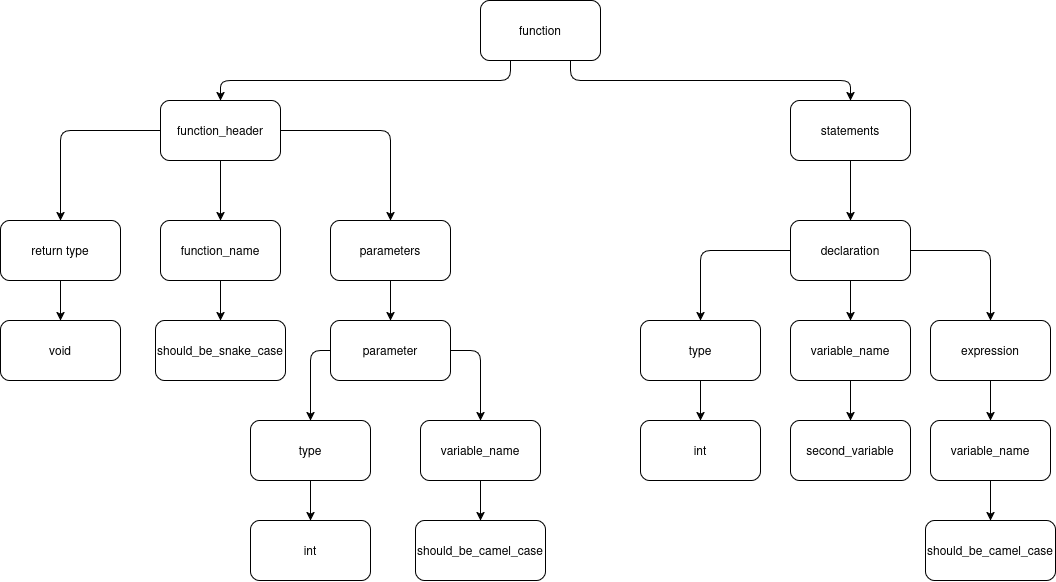
\includegraphics[scale=0.40]{fig/ast_example.png}
    \caption{AST example}
\end{figure}

This AST contains a lot of information about the program structure and allows you to distinguish between variable and function names.
\footnote{
    Depending on the grammar and language, this differentiation may not always be possible on the generated AST. 
    For example in JavaScript, functions can be passed as parameters into other functions: 
    \lstinline{function\_a(function\_b, variable\_a)}.
    The implemented LR(1) parser is not able to differentiate between the types of the parameters in this case.}. 

The following code should give a general idea of how transformations could be implemented on the AST. 
The API of \verb|gp-modifiable-ast| is different from this example.

\begin{lstlisting}[language=Java, caption=Example of transformation]
    AST ast = parser.parse("example.java");
    List<ASTNode> nodes = ast.find("variable_name");
    renameToCamelCase(nodes);
    ast.transformBackToSourceCode();
\end{lstlisting}

This transformation would result in the following code.

\begin{lstlisting}[language=Java, caption=Example of transformation]
void should_be_snake_case(int shouldBeCamelCase) {
    int secondParam = firstParam;
}
\end{lstlisting}

This example should illustrate why rewritable abstract syntax trees can be a useful tool for software development, 
because they allow a wide range of refactorings by providing access to different pieces of information about the program structure.

\subsection{Related work}

The library implemented for this thesis (\verb|gp-modifiable-ast|) has similarities to common parser generators 
such as SableCC \cite{sablecc}, ANTLR \cite{antlr}, GNU Bison \cite{gnu-bison} and others.

There are custom parsers like Esprima \cite{esprima} that can generate a modifiable AST for JavaScript sources, 
but these are limited to a specific programming language.

\verb|gp-modifiable-ast| is able to preserve the original formatting as much as possible and 
can be defined for any grammar that can be parsed by an LR(1) parser.

This work is based on the conference paper by Jeffrey L. Overbey and Ralph E. Johnson with the title 
"Generating Rewritable Abstract Syntax Trees" \cite{GeneratingRewritableAST}.
This paper defines a possible grammar definition for rewritable abstract syntax trees, which is partially implemented by \verb|gp-modifiable-ast|. 
Some of the proposed definitions of \cite{GeneratingRewritableAST} are not implemented, as they would not make sense with the
structure of \verb|gp-modifiable-ast|. The chapter \ref{chap:ast_generation} discusses which are implemented and which are not.